\documentclass{article}
\usepackage[utf8]{inputenc}

\title{Tarea3}
\author{Esteban Marulanda Ardila }
\date{Septiembre 2020}

\usepackage{natbib}
\usepackage{graphicx}

\begin{document}

\maketitle

\section{}

En la figura 1 se evidencia lo que ya se
conoce respecto a un oscilador armónico,
independientemente de su frecuencia o
condiciones iniciales, la posición de este
realiza un movimiento periódico con amplitud
constante en el tiempo.

\begin{figure}[h!]
\centering
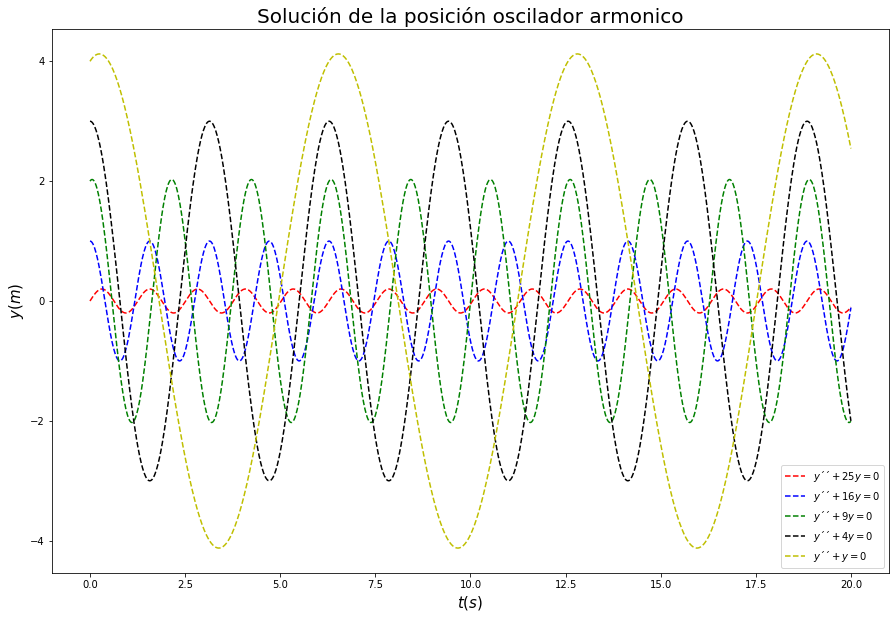
\includegraphics[width=12cm,height=7cm]{output_1_1.png}
\caption{Posición vs tiempo en un oscilador armónico}
\label{}
\end{figure}

\newline 
\noindent En el gráfico 2 muestra que para los diferentes parámetros, el espacio de fase de un osciladores armónico es una elipse, cuyos eje menor y mayor dependen de los parámetros iniciales dados al oscilador armónico. Por otro lado, que las trayectorias en el espacio de fase sean cerradas evidencia lo que ya se dijo en la anterior gráfica, el movimiento es periódico. 
\newline
\newline
\newline

\begin{figure}[h!]
\centering
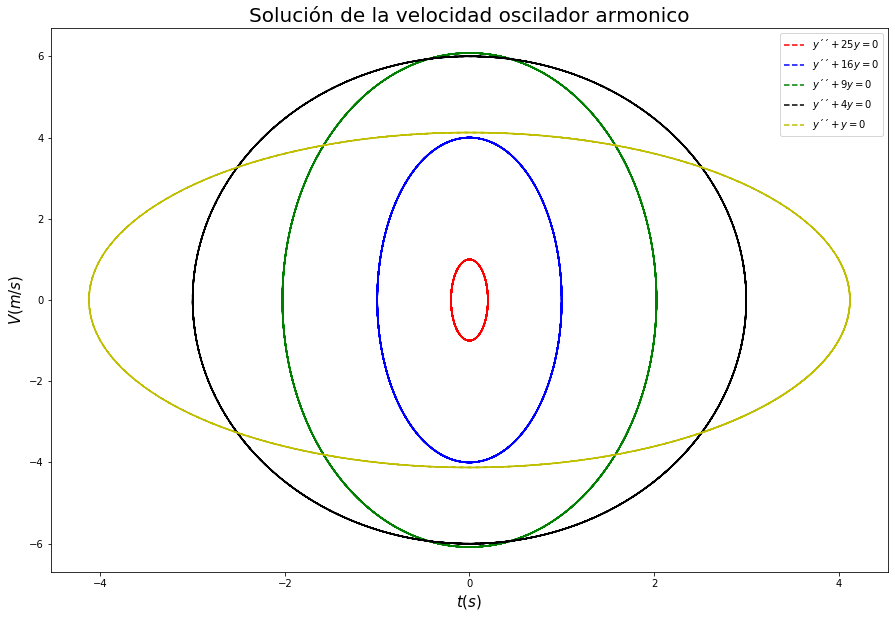
\includegraphics[width=12cm,height=7cm]{output_3_1.png}
\caption{Posición vs tiempo en un oscilador armónico para el caso subamortiguado}
\label{fig:universe}
\end{figure}

\noindent A diferencia del oscilador armónico, el factor de amortiguamiento ($\Gamma$) hace que oscilador se detenga (o 'pierda' la suficiente energía como para no evidenciar un movimiento apreciable). De la solución para los 5 conjuntos de parámetros la figura 3 muestra que dependiendo de $\Gamma$ la amortiguación es mayor o menor, esto es la amplitud del oscilador decrece más rápido en el tiempo.
\newline
\newline


\begin{figure}[h!]
\centering
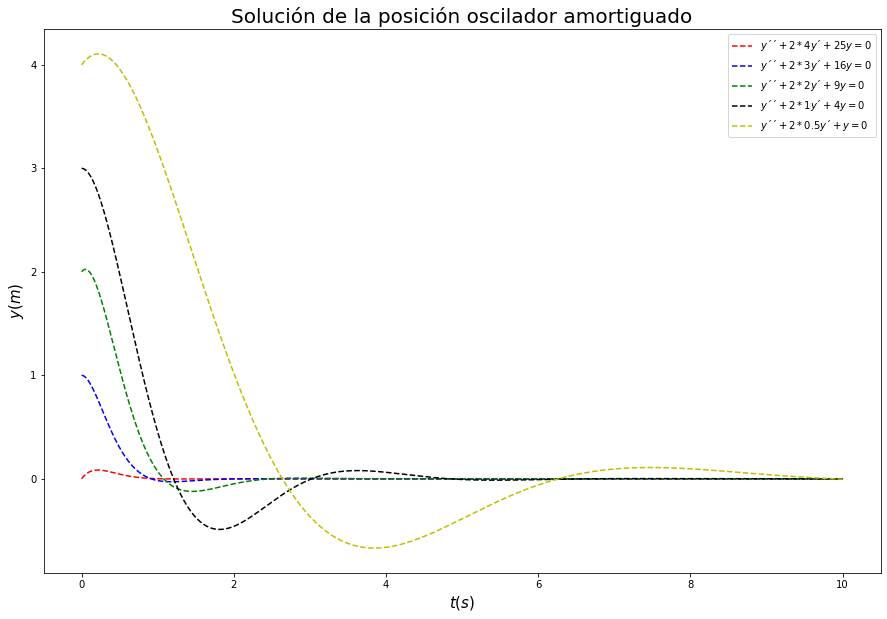
\includegraphics[width=12cm,height=7cm]{output_5_1.png}
\caption{The Universe}
\label{fig:universe}
\end{figure}

Como se discutió antes, el oscilador amortiguado tiene la característica, de que su amplitud decrezca en el tiempo, en la figura 4 se muestra  las trayectorias en el espacio de fase para los diferentes parámetros tienden todas a un mismo punto, esto  es el reposo, por eso todas tienden a $V=0$.


\begin{figure}[h!]
\centering
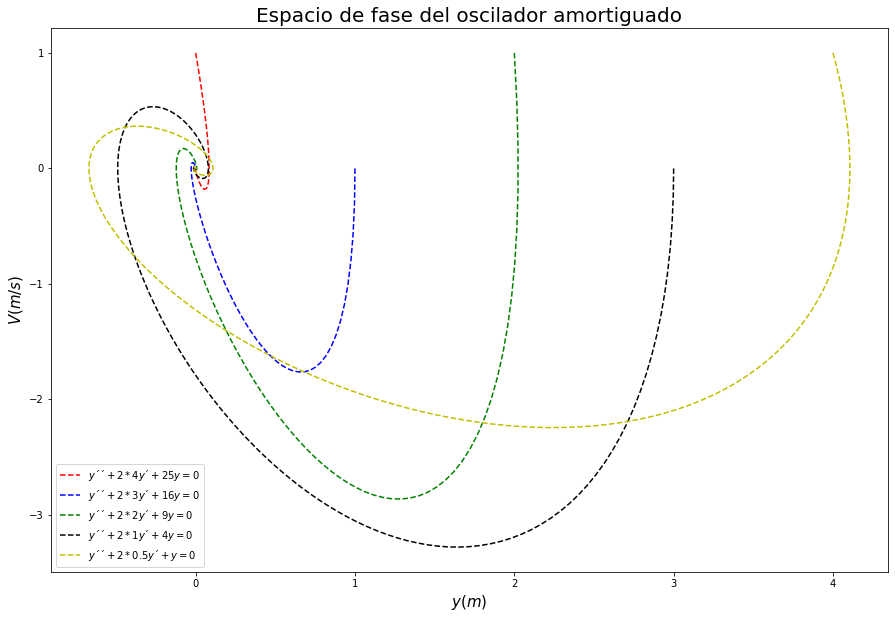
\includegraphics[width=12cm,height=7cm]{output_7_1.png}
\caption{Espacio de fase de un oscilador amortiguado para el caso subamortiguado}
\label{fig:universe}
\end{figure}
\end{document}

